% Options for packages loaded elsewhere
\PassOptionsToPackage{unicode}{hyperref}
\PassOptionsToPackage{hyphens}{url}
%
\documentclass[
  oneside]{book}
\usepackage{amsmath,amssymb}
\usepackage{lmodern}
\usepackage{iftex}
\ifPDFTeX
  \usepackage[T1]{fontenc}
  \usepackage[utf8]{inputenc}
  \usepackage{textcomp} % provide euro and other symbols
\else % if luatex or xetex
  \usepackage{unicode-math}
  \defaultfontfeatures{Scale=MatchLowercase}
  \defaultfontfeatures[\rmfamily]{Ligatures=TeX,Scale=1}
\fi
% Use upquote if available, for straight quotes in verbatim environments
\IfFileExists{upquote.sty}{\usepackage{upquote}}{}
\IfFileExists{microtype.sty}{% use microtype if available
  \usepackage[]{microtype}
  \UseMicrotypeSet[protrusion]{basicmath} % disable protrusion for tt fonts
}{}
\makeatletter
\@ifundefined{KOMAClassName}{% if non-KOMA class
  \IfFileExists{parskip.sty}{%
    \usepackage{parskip}
  }{% else
    \setlength{\parindent}{0pt}
    \setlength{\parskip}{6pt plus 2pt minus 1pt}}
}{% if KOMA class
  \KOMAoptions{parskip=half}}
\makeatother
\usepackage{xcolor}
\IfFileExists{xurl.sty}{\usepackage{xurl}}{} % add URL line breaks if available
\IfFileExists{bookmark.sty}{\usepackage{bookmark}}{\usepackage{hyperref}}
\hypersetup{
  pdftitle={Data Science \& Machine Learning},
  pdfauthor={Dieter Greipl},
  hidelinks,
  pdfcreator={LaTeX via pandoc}}
\urlstyle{same} % disable monospaced font for URLs
\usepackage{color}
\usepackage{fancyvrb}
\newcommand{\VerbBar}{|}
\newcommand{\VERB}{\Verb[commandchars=\\\{\}]}
\DefineVerbatimEnvironment{Highlighting}{Verbatim}{commandchars=\\\{\}}
% Add ',fontsize=\small' for more characters per line
\usepackage{framed}
\definecolor{shadecolor}{RGB}{248,248,248}
\newenvironment{Shaded}{\begin{snugshade}}{\end{snugshade}}
\newcommand{\AlertTok}[1]{\textcolor[rgb]{0.94,0.16,0.16}{#1}}
\newcommand{\AnnotationTok}[1]{\textcolor[rgb]{0.56,0.35,0.01}{\textbf{\textit{#1}}}}
\newcommand{\AttributeTok}[1]{\textcolor[rgb]{0.77,0.63,0.00}{#1}}
\newcommand{\BaseNTok}[1]{\textcolor[rgb]{0.00,0.00,0.81}{#1}}
\newcommand{\BuiltInTok}[1]{#1}
\newcommand{\CharTok}[1]{\textcolor[rgb]{0.31,0.60,0.02}{#1}}
\newcommand{\CommentTok}[1]{\textcolor[rgb]{0.56,0.35,0.01}{\textit{#1}}}
\newcommand{\CommentVarTok}[1]{\textcolor[rgb]{0.56,0.35,0.01}{\textbf{\textit{#1}}}}
\newcommand{\ConstantTok}[1]{\textcolor[rgb]{0.00,0.00,0.00}{#1}}
\newcommand{\ControlFlowTok}[1]{\textcolor[rgb]{0.13,0.29,0.53}{\textbf{#1}}}
\newcommand{\DataTypeTok}[1]{\textcolor[rgb]{0.13,0.29,0.53}{#1}}
\newcommand{\DecValTok}[1]{\textcolor[rgb]{0.00,0.00,0.81}{#1}}
\newcommand{\DocumentationTok}[1]{\textcolor[rgb]{0.56,0.35,0.01}{\textbf{\textit{#1}}}}
\newcommand{\ErrorTok}[1]{\textcolor[rgb]{0.64,0.00,0.00}{\textbf{#1}}}
\newcommand{\ExtensionTok}[1]{#1}
\newcommand{\FloatTok}[1]{\textcolor[rgb]{0.00,0.00,0.81}{#1}}
\newcommand{\FunctionTok}[1]{\textcolor[rgb]{0.00,0.00,0.00}{#1}}
\newcommand{\ImportTok}[1]{#1}
\newcommand{\InformationTok}[1]{\textcolor[rgb]{0.56,0.35,0.01}{\textbf{\textit{#1}}}}
\newcommand{\KeywordTok}[1]{\textcolor[rgb]{0.13,0.29,0.53}{\textbf{#1}}}
\newcommand{\NormalTok}[1]{#1}
\newcommand{\OperatorTok}[1]{\textcolor[rgb]{0.81,0.36,0.00}{\textbf{#1}}}
\newcommand{\OtherTok}[1]{\textcolor[rgb]{0.56,0.35,0.01}{#1}}
\newcommand{\PreprocessorTok}[1]{\textcolor[rgb]{0.56,0.35,0.01}{\textit{#1}}}
\newcommand{\RegionMarkerTok}[1]{#1}
\newcommand{\SpecialCharTok}[1]{\textcolor[rgb]{0.00,0.00,0.00}{#1}}
\newcommand{\SpecialStringTok}[1]{\textcolor[rgb]{0.31,0.60,0.02}{#1}}
\newcommand{\StringTok}[1]{\textcolor[rgb]{0.31,0.60,0.02}{#1}}
\newcommand{\VariableTok}[1]{\textcolor[rgb]{0.00,0.00,0.00}{#1}}
\newcommand{\VerbatimStringTok}[1]{\textcolor[rgb]{0.31,0.60,0.02}{#1}}
\newcommand{\WarningTok}[1]{\textcolor[rgb]{0.56,0.35,0.01}{\textbf{\textit{#1}}}}
\usepackage{longtable,booktabs,array}
\usepackage{calc} % for calculating minipage widths
% Correct order of tables after \paragraph or \subparagraph
\usepackage{etoolbox}
\makeatletter
\patchcmd\longtable{\par}{\if@noskipsec\mbox{}\fi\par}{}{}
\makeatother
% Allow footnotes in longtable head/foot
\IfFileExists{footnotehyper.sty}{\usepackage{footnotehyper}}{\usepackage{footnote}}
\makesavenoteenv{longtable}
\usepackage{graphicx}
\makeatletter
\def\maxwidth{\ifdim\Gin@nat@width>\linewidth\linewidth\else\Gin@nat@width\fi}
\def\maxheight{\ifdim\Gin@nat@height>\textheight\textheight\else\Gin@nat@height\fi}
\makeatother
% Scale images if necessary, so that they will not overflow the page
% margins by default, and it is still possible to overwrite the defaults
% using explicit options in \includegraphics[width, height, ...]{}
\setkeys{Gin}{width=\maxwidth,height=\maxheight,keepaspectratio}
% Set default figure placement to htbp
\makeatletter
\def\fps@figure{htbp}
\makeatother
\setlength{\emergencystretch}{3em} % prevent overfull lines
\providecommand{\tightlist}{%
  \setlength{\itemsep}{0pt}\setlength{\parskip}{0pt}}
\setcounter{secnumdepth}{5}

%\usepackage{booktabs}
%\usepackage{longtable}
%\usepackage[bf,singlelinecheck=off]{caption}

%\usepackage{Alegreya}
%\usepackage[scale=.8]{sourcecodepro}

%\usepackage[a4paper, top=1cm, bottom=1cm ]{geometry}
%\geometry{a4paper,hmargin={2cm,1.5cm},}
\usepackage[a4paper,hmargin={2cm,1.5cm}, vmargin={1.5cm,1.5cm} ]{geometry}

%---------------------------------- Seitenlayout
\textwidth 160mm
\textheight 240mm
\topmargin=-15mm

\setlength\oddsidemargin{(\paperwidth-\textwidth)/2 - 1in}
\setlength\topmargin{(\paperheight-\textheight
-\headheight-\headsep-\footskip)/2 - 1in}

% Kopfzeile unterstreichen
\usepackage[%
headsepline,
%footsepline % no separation line for page number
]{scrlayer-scrpage}

\setcounter{tocdepth}{3}
\setcounter{secnumdepth}{4}





\ifLuaTeX
  \usepackage{selnolig}  % disable illegal ligatures
\fi
\usepackage[]{natbib}
\bibliographystyle{apalike}

\title{Data Science \& Machine Learning}
\author{Dieter Greipl}
\date{2022-01-22}

\begin{document}
\maketitle

{
\setcounter{tocdepth}{1}
\tableofcontents
}
\hypertarget{willkommen}{%
\chapter*{Willkommen}\label{willkommen}}
\addcontentsline{toc}{chapter}{Willkommen}

Dieses Skript entstand (und entsteht) aus meinen Lehrveranstaltungen rund um das Thema \textbf{Data Science \& Machine Learning}. Die Inhalte richten sich an Studierende, die erste Schritte auf das KI -Spielfeld wagen und das Potential von datengetriebenen Lösungsverfahren verstehen wollen.

Insofern richtet sich die Darstellung an Studierende mit vertieftem Interesse an KI, die einen für Studierende angemessenes Vorwissen im Bereich Mathematik mitbringen. Vorkenntnisse im Bereich der Programmierung sind nicht nötig, aber natürlich hilfreich.

Ich habe mich bemüht, zahlreiche Übungsbeispiele und Youtube-Videos einzubauen. Viele Themen lassen sich so besser darstellen. Sofern es Medien im Netz gibt, die die Sachverhalte gut darstellen, werde ich entsprechenden Links einbauen. Der Autor muss ja nicht der Meinung sein, alles besser zu können. Gleichwohl darf dadurch der rote Faden nicht verloren gehen.

\hypertarget{vorbereitungen}{%
\section{Vorbereitungen}\label{vorbereitungen}}

Dieses Skript ist als Unterlage für zahlreichen praktische Übungen mit Python angelegt. Ich werde hierzu \href{https://colab.research.google.com/}{\textbf{Colab-Notebooks}} verwenden. Sie brauchen hierzu ein \textbf{Google-Konto}.

Noch einige Hinweise an Studierende meiner Module:

\begin{itemize}
\tightlist
\item
  Die folgende Youtube-Playlist kann zur Vertiefung einzelner Stoffteile nutzen: \href{https://youtube.com/playlist?list=PLfGN40VwjduJPvtP9QUjC0rjM6-ePT9bg}{Youtube Playlist}
\item
  Wenige Passagen in diesem Skript sind eventuell in englischer Sprache gehalten.
\item
  Dieses Skript

  \begin{itemize}
  \tightlist
  \item
    befindet sich in Teilen im Aufbau, leichte Fehler sind also möglich (und wahrscheinlich - für Hinweise bin ich dankbar)
  \item
    geht nach der Prüfung off-line
  \end{itemize}
\end{itemize}

\hypertarget{python---quickstart}{%
\chapter{Python - Quickstart}\label{python---quickstart}}

\hypertarget{colab-notebooks}{%
\section{Colab-Notebooks}\label{colab-notebooks}}

\hypertarget{hallo-welt}{%
\section{Hallo Welt}\label{hallo-welt}}

\begin{Shaded}
\begin{Highlighting}[]
\BuiltInTok{print}\NormalTok{(}\StringTok{"Hallo Welt"}\NormalTok{)}
\end{Highlighting}
\end{Shaded}

Ausgabe:

\begin{verbatim}
#> Hallo Welt
\end{verbatim}

\hypertarget{variablen}{%
\section{Variablen}\label{variablen}}

Variablen sind Platzhalter für Werte, wir sprechen vom \emph{Wert einer Variable}. Im nachfolgendem Beispiel wird der Variable mit dem Namen \texttt{x}in Zeile 1 der Wert 1 zugewiesen. Variablen haben immer einen Namen. Einen Wert erhalten sie erst durch eine sog. Zuweisung (wie in Zeile 1). In Zeile 2 drucken wir den Wert aus. Führen Sie also folgende Phython-Befehle aus:

\begin{Shaded}
\begin{Highlighting}[]
\NormalTok{x }\OperatorTok{=} \DecValTok{1}
\BuiltInTok{print}\NormalTok{(x)}
\end{Highlighting}
\end{Shaded}

\begin{quote}
Die erstmalige Zuweisung eines Wertes an eine Variable heißt Initialisierung.
\end{quote}

\hypertarget{datentypen}{%
\section{Datentypen}\label{datentypen}}

\hypertarget{datentyp-zahlen}{%
\subsection{Datentyp ``Zahlen''}\label{datentyp-zahlen}}

\hypertarget{ganze-zahlen-und-rationale-zahlen}{%
\subsubsection{Ganze Zahlen und rationale Zahlen}\label{ganze-zahlen-und-rationale-zahlen}}

Zahlen sind recht einfach zu verstehen, wir haben ja oben schon einige Beispiele gesehen. Hier nochmal eine Zusammenfassung wichtiger Beispiele mit rationalen Zahlen: 

\begin{Shaded}
\begin{Highlighting}[]
\NormalTok{a }\OperatorTok{=} \DecValTok{2}
\NormalTok{b }\OperatorTok{=} \DecValTok{1}\OperatorTok{/}\DecValTok{3}
\NormalTok{c }\OperatorTok{=} \FloatTok{1.1}
\CommentTok{\# Funktionen}
\NormalTok{d }\OperatorTok{=}\NormalTok{ a }\OperatorTok{+}\NormalTok{ b}\OperatorTok{;} \BuiltInTok{print}\NormalTok{(d)}
\NormalTok{d }\OperatorTok{=}\NormalTok{ a }\OperatorTok{{-}}\NormalTok{ b}\OperatorTok{;} \BuiltInTok{print}\NormalTok{(d)}
\NormalTok{d }\OperatorTok{=}\NormalTok{ a }\OperatorTok{*}\NormalTok{ b}\OperatorTok{;} \BuiltInTok{print}\NormalTok{(d)}
\NormalTok{d }\OperatorTok{=}\NormalTok{ a }\OperatorTok{/}\NormalTok{ b}\OperatorTok{;} \BuiltInTok{print}\NormalTok{(d)}
\end{Highlighting}
\end{Shaded}

\hypertarget{datentyp-strings}{%
\subsection{Datentyp ``Strings''}\label{datentyp-strings}}

Zeichenketten sind ebenfalls recht einfach zu verstehen. Führen Sie folgendes Beispiel aus:

\begin{Shaded}
\begin{Highlighting}[]
\NormalTok{vorname }\OperatorTok{=} \StringTok{"Hans"}
\NormalTok{nachname }\OperatorTok{=} \StringTok{\textquotesingle{}Huber\textquotesingle{}}
\NormalTok{name }\OperatorTok{=}\NormalTok{ vorname }\OperatorTok{+} \StringTok{", "} \OperatorTok{+}\NormalTok{ nachname}
\BuiltInTok{print}\NormalTok{(name)}
\end{Highlighting}
\end{Shaded}

\hypertarget{f-strings}{%
\subsubsection{f-Strings}\label{f-strings}}

Statt eine zusammengesetzte Zeichenkette mit dem ``+'' - Operator auf zubauen, kann ein sogenannter f-String verwendet werden (siehe Zeile 3). f-Strings bringen für uns keine neue Funktion, machen aber die Verknüpfung von Strings einfacher.

\begin{Shaded}
\begin{Highlighting}[]
\NormalTok{vorname }\OperatorTok{=} \StringTok{"Hans"}
\NormalTok{nachname }\OperatorTok{=} \StringTok{\textquotesingle{}Huber\textquotesingle{}}
\NormalTok{name }\OperatorTok{=} \SpecialStringTok{f"}\SpecialCharTok{\{}\NormalTok{vorname}\SpecialCharTok{\}}\SpecialStringTok{, }\SpecialCharTok{\{}\NormalTok{nachname}\SpecialCharTok{\}}\SpecialStringTok{"}
\BuiltInTok{print}\NormalTok{(name)}
\end{Highlighting}
\end{Shaded}

\hypertarget{datentyp-boolean}{%
\subsection{Datentyp ``Boolean''}\label{datentyp-boolean}}

Es gibt in der Theorie unendlich viele Zahlen und Zeichenketten, aber nur zwei Wahrheitswerte: wahr oder falsch. In Phython: \texttt{True}und \texttt{False}

\begin{Shaded}
\begin{Highlighting}[]
\NormalTok{z1 }\OperatorTok{=} \VariableTok{False}\OperatorTok{;}
\BuiltInTok{print}\NormalTok{ (z1)}
\BuiltInTok{print}\NormalTok{( }\BuiltInTok{type}\NormalTok{(z1) )}\OperatorTok{;}

\NormalTok{z2 }\OperatorTok{=} \DecValTok{1} \OperatorTok{\textless{}} \DecValTok{4}\OperatorTok{;}
\BuiltInTok{print}\NormalTok{( z2 )}\OperatorTok{;}
\BuiltInTok{print}\NormalTok{( }\BuiltInTok{type}\NormalTok{(z2) )}\OperatorTok{;}

\BuiltInTok{print}\NormalTok{ (}\StringTok{"z1 and z2:"}\NormalTok{, z1 }\KeywordTok{and}\NormalTok{ z2)}\OperatorTok{;}
\BuiltInTok{print}\NormalTok{ (}\StringTok{"z1 or z2:"}\NormalTok{, z1 }\KeywordTok{or}\NormalTok{ z2)}\OperatorTok{;}
\end{Highlighting}
\end{Shaded}

\hypertarget{operatoren}{%
\section{Operatoren}\label{operatoren}}

Die Bildschirmabzüge dieses Kapitels sind der Webseite \url{https://www.w3schools.com/python/python_operators.asp} entnommen. Erarbeiten Sie sich die Operatoren selbst in kleinen Programmen, so wie wir das zu Zahlen bereits oben gemacht haben.

\hypertarget{arithmetische-operatoren}{%
\subsection{Arithmetische Operatoren}\label{arithmetische-operatoren}}

\begin{figure}
\centering
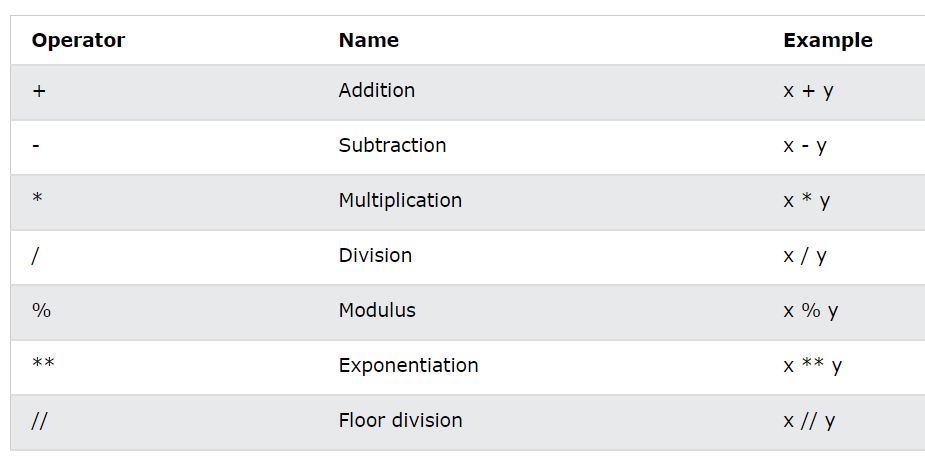
\includegraphics{assets/python.assets/bild1.png}
\caption{bild1}
\end{figure}

\hypertarget{vergleichsoperatoren}{%
\subsection{Vergleichsoperatoren}\label{vergleichsoperatoren}}

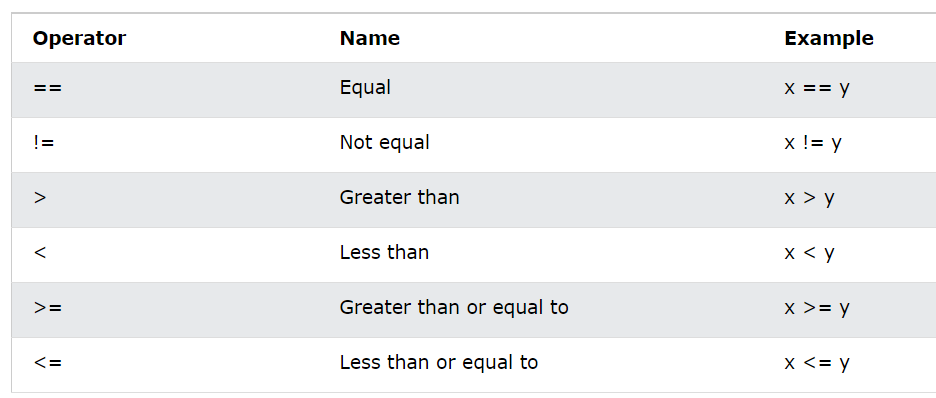
\includegraphics{01-python.assets/image (187).png}

\hypertarget{logische-operatoren}{%
\subsection{Logische Operatoren}\label{logische-operatoren}}

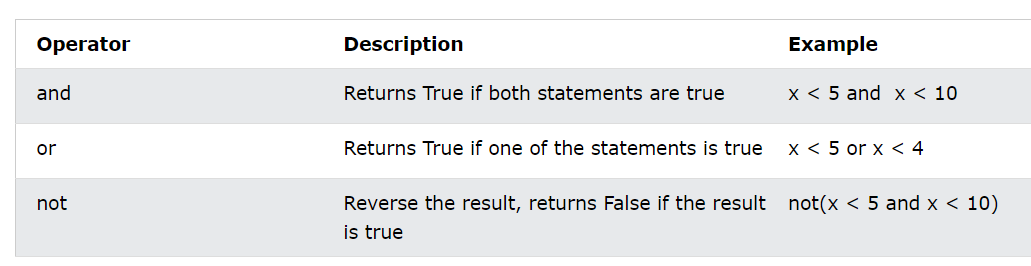
\includegraphics{assets/python.assets/image (188).png}

\hypertarget{datentypen-in-der-uxfcbersicht}{%
\section{Datentypen in der Übersicht}\label{datentypen-in-der-uxfcbersicht}}

Nachfolgendes Programmstück beschreibt exemplarisch die nun bekannten Datentypen. Mit \texttt{type()} kann man sich den Datentyp einer Variable ausgeben lassen (oft hilfreich!)

\begin{Shaded}
\begin{Highlighting}[]
\NormalTok{x }\OperatorTok{=} \DecValTok{1}\OperatorTok{;} 
\BuiltInTok{print}\NormalTok{( }\SpecialStringTok{f"1 : }\SpecialCharTok{\{}\BuiltInTok{type}\NormalTok{(x)}\SpecialCharTok{\}}\SpecialStringTok{"}\NormalTok{)}

\NormalTok{x }\OperatorTok{=} \FloatTok{1.1}\OperatorTok{;} 
\BuiltInTok{print}\NormalTok{( }\SpecialStringTok{f"1.1 : }\SpecialCharTok{\{}\BuiltInTok{type}\NormalTok{(x)}\SpecialCharTok{\}}\SpecialStringTok{"}\NormalTok{)}

\NormalTok{x }\OperatorTok{=} \DecValTok{4}\OperatorTok{/}\DecValTok{2}\OperatorTok{;} 
\BuiltInTok{print}\NormalTok{( }\SpecialStringTok{f"4/2 : }\SpecialCharTok{\{}\BuiltInTok{type}\NormalTok{(x)}\SpecialCharTok{\}}\SpecialStringTok{"}\NormalTok{)}

\NormalTok{x }\OperatorTok{=} \StringTok{\textquotesingle{}String\textquotesingle{}}\OperatorTok{;} 
\BuiltInTok{print}\NormalTok{( }\SpecialStringTok{f"\textquotesingle{}String\textquotesingle{} : }\SpecialCharTok{\{}\BuiltInTok{type}\NormalTok{(x)}\SpecialCharTok{\}}\SpecialStringTok{"}\NormalTok{)}

\NormalTok{x }\OperatorTok{=}\NormalTok{ [}\DecValTok{1}\NormalTok{,}\DecValTok{2}\NormalTok{,}\DecValTok{4}\NormalTok{]}\OperatorTok{;} 
\BuiltInTok{print}\NormalTok{( }\SpecialStringTok{f"[1,2,3] : }\SpecialCharTok{\{}\BuiltInTok{type}\NormalTok{(x)}\SpecialCharTok{\}}\SpecialStringTok{"}\NormalTok{)}

\NormalTok{x }\OperatorTok{=}\NormalTok{ (}\DecValTok{1}\NormalTok{,}\DecValTok{2}\NormalTok{)}\OperatorTok{;}
\BuiltInTok{print}\NormalTok{( }\SpecialStringTok{f"(1,2) : }\SpecialCharTok{\{}\BuiltInTok{type}\NormalTok{(x)}\SpecialCharTok{\}}\SpecialStringTok{"}\NormalTok{)}

\NormalTok{x }\OperatorTok{=} \DecValTok{1} \OperatorTok{\textless{}} \OperatorTok{{-}}\DecValTok{3}
\BuiltInTok{print}\NormalTok{( }\SpecialStringTok{f"False : }\SpecialCharTok{\{}\BuiltInTok{type}\NormalTok{(x)}\SpecialCharTok{\}}\SpecialStringTok{"}\NormalTok{)}
\end{Highlighting}
\end{Shaded}

\hypertarget{zusammenfassung}{%
\subsection{Zusammenfassung}\label{zusammenfassung}}

\begin{longtable}[]{@{}lll@{}}
\toprule
Eingebauter Datentyp & Kürzel & Beispiele \\
\midrule
\endhead
Text (Strings) & str & \texttt{x\ =\ "Haw-Landshut"} \\
Zahlen (Numerisch) & int, float & \texttt{x\ =\ 1} oder \texttt{x\ =\ 1.1} \\
Listen (Arrays) & list & \texttt{x\ =\ {[}1,2,3{]}} \\
Tupel & tuple & \texttt{x\ =\ (1,2)} \\
Wahrheitswerte & bool & \texttt{x\ =\ (1\ \textless{}\ 3)} \\
\bottomrule
\end{longtable}

\hypertarget{daten}{%
\chapter{Daten}\label{daten}}

\hypertarget{der-iris-datensatz}{%
\section{Der Iris-Datensatz}\label{der-iris-datensatz}}

Der Iris-Datensatz enthält Messungen von jeweils 50 Blüten zu drei verschiedenen Lilien-Arten (setosa, versicolor, virginica)

\begin{figure}
\centering
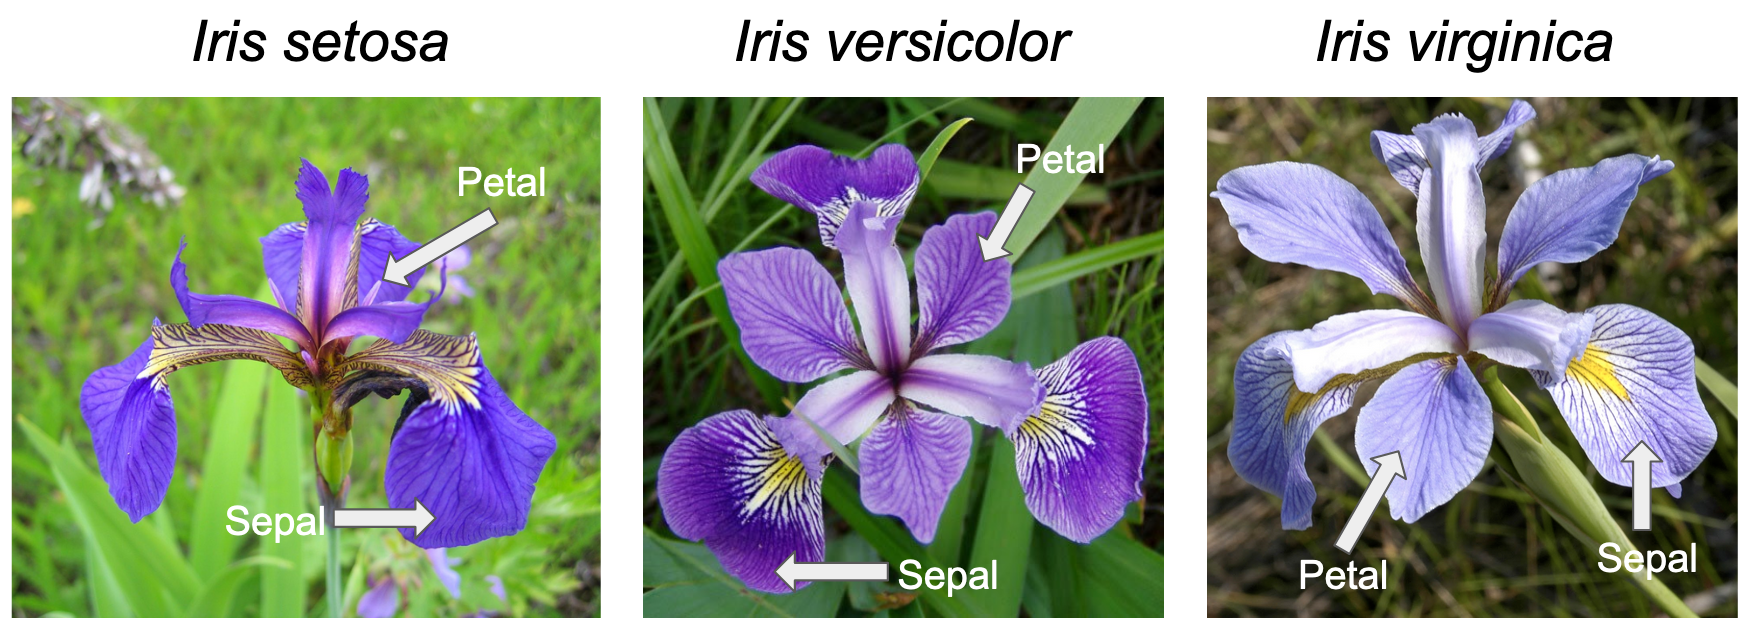
\includegraphics{assets/daten.assets/Download.png}
\caption{Download}
\end{figure}

Gemessen werden pro \href{https://de.wikipedia.org/wiki/Bl\%C3\%BCte}{Blüte}in cm 

\begin{itemize}
\tightlist
\item
  die Länge und Breite des Kronblattes (Petalum, petal) sowie 
\item
  die Länge und Breite des Kelchblattes (Sepalum, sepal)
\end{itemize}

\begin{figure}
\centering
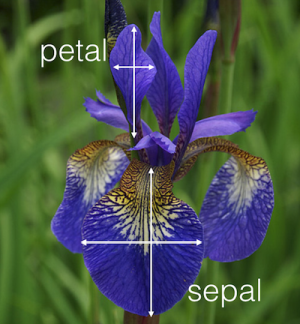
\includegraphics{assets/daten.assets/image_messung-16426070933692.png}
\caption{image (190)}
\end{figure}

\hypertarget{datensatz}{%
\subsection{Datensatz}\label{datensatz}}

Folgender - in der Community wohlbekannter - Datensatz liegt uns vor (Sie finden die Daten \href{https://syncandshare.lrz.de/getlink/fi89kxTJ5yLRaW5mnpyrofVK/Iris_p.xlsx}{hier}).

\begin{figure}
\centering
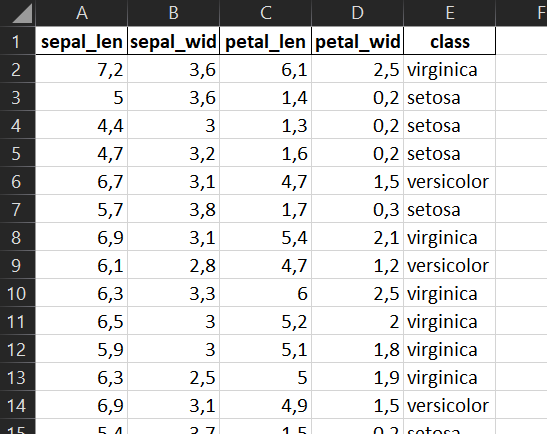
\includegraphics{assets/daten.assets/image-20211209101425856-16426070878651.png}
\caption{Iris-Datensatz}
\end{figure}

\hypertarget{datentypen-1}{%
\section{Datentypen}\label{datentypen-1}}

\hypertarget{elementare-datentypen}{%
\subsection{Elementare Datentypen}\label{elementare-datentypen}}

\hypertarget{zahlen}{%
\subsubsection{Zahlen}\label{zahlen}}

\hypertarget{strings}{%
\subsubsection{Strings}\label{strings}}

\hypertarget{logische-werte}{%
\subsubsection{Logische Werte}\label{logische-werte}}

\hypertarget{elementare-datentypen-in-python}{%
\subsubsection{Elementare Datentypen in Python}\label{elementare-datentypen-in-python}}

\hypertarget{komplexe-datentypen}{%
\subsection{Komplexe Datentypen}\label{komplexe-datentypen}}

\hypertarget{datum}{%
\subsubsection{Datum}\label{datum}}

\hypertarget{uhrzeit}{%
\subsubsection{Uhrzeit}\label{uhrzeit}}

\hypertarget{bilder}{%
\subsubsection{Bilder}\label{bilder}}

\hypertarget{komplexe-datentypen-in-python}{%
\subsubsection{Komplexe Datentypen in Python}\label{komplexe-datentypen-in-python}}

\hypertarget{skalenniveaus}{%
\section{Skalenniveaus}\label{skalenniveaus}}

\hypertarget{uxfcberblick}{%
\subsection{Überblick}\label{uxfcberblick}}

\begin{longtable}[]{@{}
  >{\raggedright\arraybackslash}p{(\columnwidth - 8\tabcolsep) * \real{0.0563}}
  >{\raggedright\arraybackslash}p{(\columnwidth - 8\tabcolsep) * \real{0.0915}}
  >{\raggedright\arraybackslash}p{(\columnwidth - 8\tabcolsep) * \real{0.4225}}
  >{\raggedright\arraybackslash}p{(\columnwidth - 8\tabcolsep) * \real{0.1268}}
  >{\raggedright\arraybackslash}p{(\columnwidth - 8\tabcolsep) * \real{0.3028}}@{}}
\toprule
\begin{minipage}[b]{\linewidth}\raggedright
Scale
\end{minipage} & \begin{minipage}[b]{\linewidth}\raggedright
Operations
\end{minipage} & \begin{minipage}[b]{\linewidth}\raggedright
Description
\end{minipage} & \begin{minipage}[b]{\linewidth}\raggedright
Statistics
\end{minipage} & \begin{minipage}[b]{\linewidth}\raggedright
Example
\end{minipage} \\
\midrule
\endhead
Nominal & \(=, \neq\) & values have no natural order; they describe unordered categories & Mode (Modus) & München, Hamburg, Essen \\
Ordinal & \(<, >\) & values have a defined order; difference of values is undefined or has no clear or meaningful definition & Median & Schulnoten, Tabellenplatz in der Bundesliga \\
Interval & \(+,-\) & differences of values have the same meaning; adding provides useful results; zero point is not naturally/globally defined & Mean & Temperatur \\
Ratio & \(\cdot , /\) & zero point is naturally defined & (Generalized) Mean & Alter \\
\bottomrule
\end{longtable}

Bemerkungen:

\begin{enumerate}
\def\labelenumi{\arabic{enumi}.}
\item
  Skalenniveaus sind nicht immer klar zuzuordnen.
\item
  Auf nominalen Datenskalen lassen sich stets \emph{künstliche Ordnungen} (und damit ordinale Datenskalen) definieren.
\item
  Bilden sie keine Mittelwerte auf Daten mit ordinalen Datenskalen!
\item
  Nominale und ordinale Datenskalen heißen auch \emph{kategorisch} oder \emph{qualitativ}.
\item
  Intervall und Ratio-Datenskalen heißen auch \emph{metrisch}.
\end{enumerate}

Ergänzend: \href{https://www.statistikpsychologie.de/skalenniveaus/}{Die fünf Skalenniveaus: Einfach und verständlich erklärt (statistikpsychologie.de)}

\hypertarget{skalenniveaus-im-iris-datensatz}{%
\subsection{Skalenniveaus im Iris-Datensatz}\label{skalenniveaus-im-iris-datensatz}}

\begin{figure}
\centering
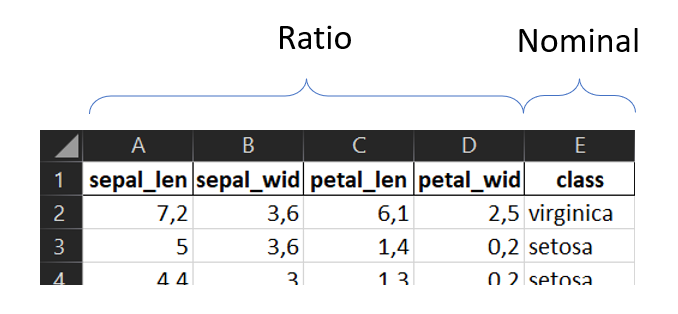
\includegraphics{assets/daten.assets/image-20211209145313372.png}
\caption{Skalenniveaus bei Iris}
\end{figure}

\hypertarget{von-nominal-zu-ordinal}{%
\paragraph{Von Nominal zu Ordinal}\label{von-nominal-zu-ordinal}}

Wir werden später folgende eindeutige Zuordnung treffen:

\begin{longtable}[]{@{}cc@{}}
\toprule
Nominaler Wert & Ordinaler Wert \\
\midrule
\endhead
setosa & 0 \\
versicolor & 1 \\
virginica & 2 \\
\bottomrule
\end{longtable}

\hypertarget{matplotlib-und-seaborn}{%
\chapter{Matplotlib und Seaborn}\label{matplotlib-und-seaborn}}

Mathplotlib (\href{https://matplotlib.org}{https://matplotlib.org/}) ist eine Sammlung von Funktionen (Bibliothek) zum Visualisieren von Daten. Wir verwenden mathplotlib zusammen mit dem ergänzenden Programmpaket Seaborn.

Wichtig: Sie müssen die folgenden beiden Zeilen stets am Beginn des Programms stehen haben.

\begin{Shaded}
\begin{Highlighting}[]
\ImportTok{import}\NormalTok{ matplotlib.pyplot }\ImportTok{as}\NormalTok{ plt}
\ImportTok{import}\NormalTok{ seaborn }\ImportTok{as}\NormalTok{ sns}
\end{Highlighting}
\end{Shaded}

\hypertarget{plots}{%
\chapter{Plots}\label{plots}}

\hypertarget{scatterplot}{%
\section{Scatterplot}\label{scatterplot}}

\begin{Shaded}
\begin{Highlighting}[]
\CommentTok{\#Scatterplot}
\ImportTok{import}\NormalTok{ matplotlib.pyplot }\ImportTok{as}\NormalTok{ plt}
\ImportTok{import}\NormalTok{ seaborn }\ImportTok{as}\NormalTok{ sns}

\NormalTok{years }\OperatorTok{=}\NormalTok{ [}\DecValTok{1950}\NormalTok{, }\DecValTok{1960}\NormalTok{, }\DecValTok{1970}\NormalTok{, }\DecValTok{1980}\NormalTok{, }\DecValTok{1990}\NormalTok{, }\DecValTok{2000}\NormalTok{, }\DecValTok{2010}\NormalTok{]}
\NormalTok{gdp }\OperatorTok{=}\NormalTok{ [}\FloatTok{33.2}\NormalTok{, }\FloatTok{543.3}\NormalTok{, }\FloatTok{1075.9}\NormalTok{, }\FloatTok{2862.5}\NormalTok{, }\FloatTok{5979.6}\NormalTok{, }\FloatTok{10289.7}\NormalTok{, }\FloatTok{14958.3}\NormalTok{]}

\NormalTok{sns.}\BuiltInTok{set}\NormalTok{()}
\NormalTok{fig,ax }\OperatorTok{=}\NormalTok{ plt.subplots(figsize}\OperatorTok{=}\NormalTok{(}\DecValTok{9}\NormalTok{, }\DecValTok{9}\NormalTok{))}
\NormalTok{ax.set\_title(}\StringTok{"Title"}\NormalTok{) }
\NormalTok{ax.set\_xlabel(}\StringTok{"x{-}axis"}\NormalTok{)}
\NormalTok{ax.set\_ylabel(}\StringTok{"y{-}axis"}\NormalTok{)}
\CommentTok{\#ax.set\_aspect(\textquotesingle{}equal\textquotesingle{})}
\CommentTok{\#ax.set\_xlim(0, 50)}
\CommentTok{\#ax.set\_ylim(0, 35)}

\NormalTok{sns.scatterplot(x}\OperatorTok{=}\NormalTok{years, y}\OperatorTok{=}\NormalTok{gdp, color}\OperatorTok{=}\StringTok{"red"}\NormalTok{, label}\OperatorTok{=}\StringTok{"My Label"}\NormalTok{)          }
\end{Highlighting}
\end{Shaded}

\begin{figure}
\centering
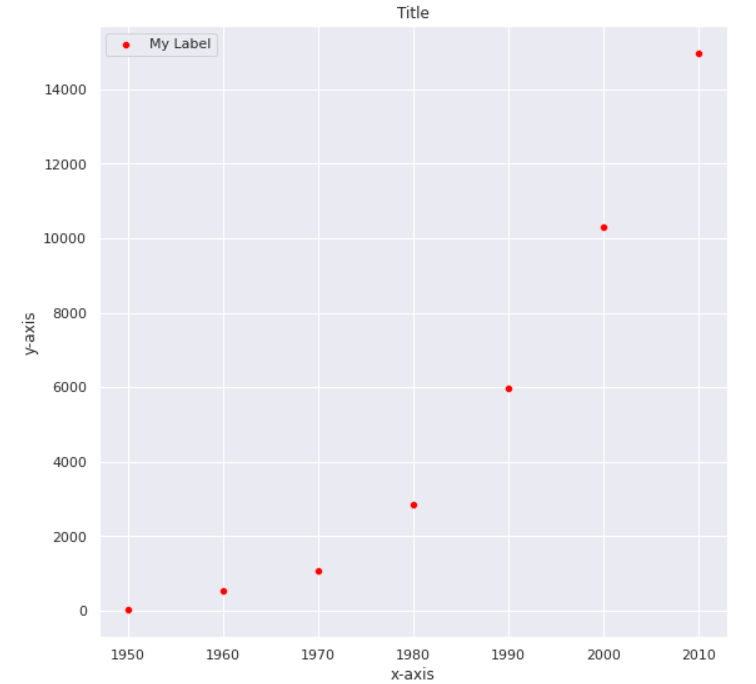
\includegraphics{readme.assets/image-20211209163345000.png}
\caption{Ausgabe}
\end{figure}

Hinweise:

\begin{itemize}
\tightlist
\item
  Zu Farben siehe : \url{https://seaborn.pydata.org/tutorial/color_palettes.html} (Vorsicht, anspruchsvoll)
\item
  Formatierung der Achsen beachten
\end{itemize}

\hypertarget{liniendiagramme}{%
\section{Liniendiagramme}\label{liniendiagramme}}

Hier ein erstes Beispiel:

\begin{Shaded}
\begin{Highlighting}[]
\CommentTok{\#Line}
\NormalTok{sns.scatterplot(x}\OperatorTok{=}\NormalTok{years, y}\OperatorTok{=}\NormalTok{gdp, color}\OperatorTok{=}\StringTok{"red"}\NormalTok{, label}\OperatorTok{=}\StringTok{"My Label"}\NormalTok{)}
\end{Highlighting}
\end{Shaded}

\begin{figure}
\centering
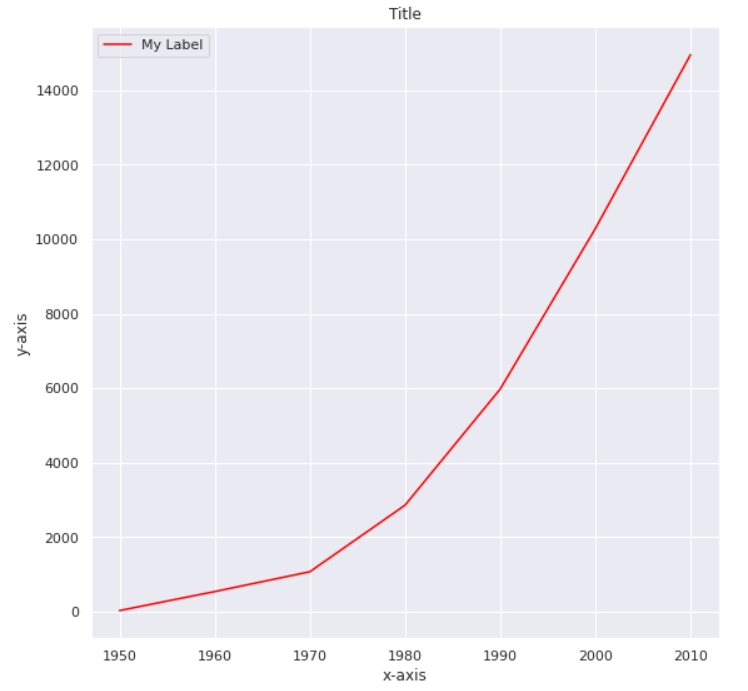
\includegraphics{readme.assets/image-20211209164634964.png}
\caption{image-20211209164634964}
\end{figure}

\hypertarget{barplot}{%
\section{Barplot}\label{barplot}}

\begin{verbatim}
sns.barplot(x=years, y=gdp, color="red", label="My Label")
\end{verbatim}

\hypertarget{histogramme}{%
\section{Histogramme}\label{histogramme}}

\begin{Shaded}
\begin{Highlighting}[]
\ImportTok{import}\NormalTok{ matplotlib.pyplot }\ImportTok{as}\NormalTok{ plt}
\ImportTok{import}\NormalTok{ seaborn }\ImportTok{as}\NormalTok{ sns}

\NormalTok{x\_werte }\OperatorTok{=}\NormalTok{  [}\DecValTok{1}\NormalTok{, }\DecValTok{2}\NormalTok{, }\DecValTok{2}\NormalTok{, }\DecValTok{3}\NormalTok{,}\DecValTok{3}\NormalTok{, }\DecValTok{4}\NormalTok{, }\DecValTok{5}\NormalTok{, }\DecValTok{6}\NormalTok{, }\DecValTok{7}\NormalTok{, }\DecValTok{8}\NormalTok{, }\DecValTok{9}\NormalTok{, }\DecValTok{10}\NormalTok{]}

\NormalTok{sns.}\BuiltInTok{set}\NormalTok{()}
\NormalTok{sns.histplot(x }\OperatorTok{=}\NormalTok{ x\_werte,}
             \CommentTok{\#binwidth=1,}
             \CommentTok{\#bins="auto",}
\NormalTok{             bins}\OperatorTok{=}\NormalTok{[}\DecValTok{0}\NormalTok{,}\DecValTok{2}\NormalTok{,}\DecValTok{5}\NormalTok{,}\DecValTok{7}\NormalTok{,}\DecValTok{10}\NormalTok{],}
\NormalTok{             kde }\OperatorTok{=} \VariableTok{False}\NormalTok{)}
\end{Highlighting}
\end{Shaded}

\begin{figure}
\centering
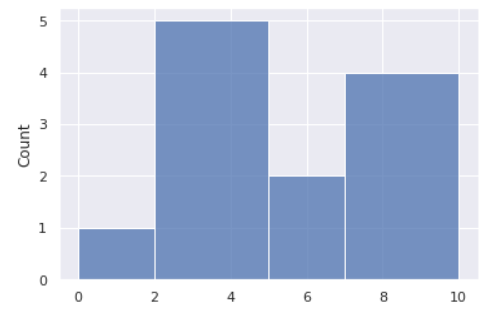
\includegraphics{readme.assets/image-20211210105040430.png}
\caption{image-20211210105040430}
\end{figure}

\hypertarget{boxplots}{%
\section{Boxplots}\label{boxplots}}

Link: \url{https://seaborn.pydata.org/generated/seaborn.boxplot.html} 

Link: \url{https://towardsdatascience.com/understanding-boxplots-5e2df7bcbd51}

\begin{figure}
\centering
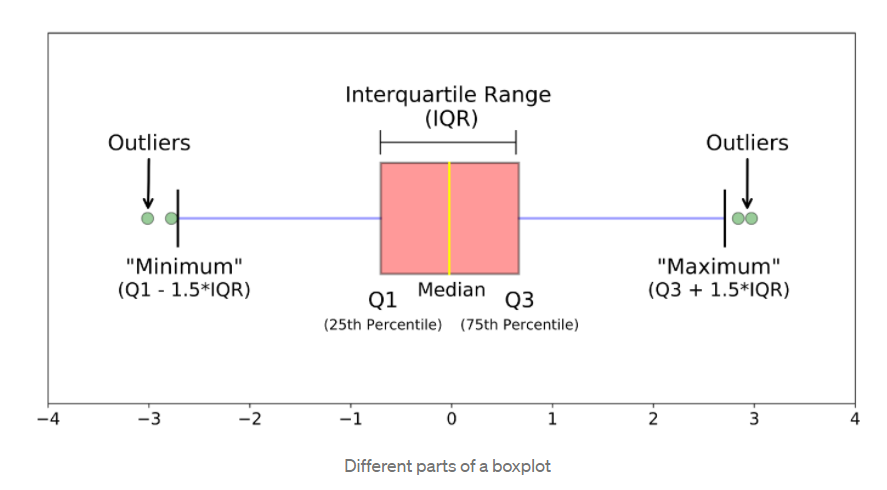
\includegraphics{readme.assets/image-20211210123539036.png}
\caption{image-20211210123539036}
\end{figure}

Vertiefung:

\href{http://rocketdatascience.org/?p=473}{Outliers, Inliers, and Other Surprises that Fly from your Data \textbar{} Rocket-Powered Data Science (rocketdatascience.org)}

\begin{Shaded}
\begin{Highlighting}[]
\ImportTok{import}\NormalTok{ matplotlib.pyplot }\ImportTok{as}\NormalTok{ plt}
\ImportTok{import}\NormalTok{ seaborn }\ImportTok{as}\NormalTok{ sns}

\NormalTok{x }\OperatorTok{=}\NormalTok{ np.arange(}\DecValTok{1}\NormalTok{,}\DecValTok{101}\NormalTok{)}
\NormalTok{x }\OperatorTok{=}\NormalTok{ np.concatenate( (x, [}\DecValTok{152}\NormalTok{] ))}

\NormalTok{percentiles }\OperatorTok{=}\NormalTok{ np.percentile( x, [}\DecValTok{0}\NormalTok{,}\DecValTok{25}\NormalTok{,}\DecValTok{50}\NormalTok{,}\DecValTok{75}\NormalTok{,}\DecValTok{100}\NormalTok{])}
\NormalTok{IQR }\OperatorTok{=}\NormalTok{ (percentiles[}\DecValTok{3}\NormalTok{] }\OperatorTok{{-}}\NormalTok{  percentiles[}\DecValTok{1}\NormalTok{])}
\BuiltInTok{print}\NormalTok{( }\StringTok{"Pericentile         : "}\NormalTok{, percentiles)}
\BuiltInTok{print}\NormalTok{( }\StringTok{"IQR                 : "}\NormalTok{, IQR)}
\BuiltInTok{print}\NormalTok{( }\StringTok{"Upper Outlier Limit : "}\NormalTok{, percentiles[}\DecValTok{3}\NormalTok{] }\OperatorTok{+} \FloatTok{1.5}\OperatorTok{*}\NormalTok{IQR)}
\NormalTok{sns.boxplot(x }\OperatorTok{=}\NormalTok{ x)}
\end{Highlighting}
\end{Shaded}

\begin{figure}
\centering
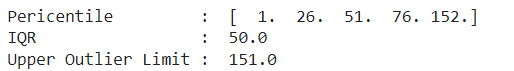
\includegraphics{readme.assets/image-20211210124842057.png}
\caption{image-20211210124842057}
\end{figure}

\begin{figure}
\centering
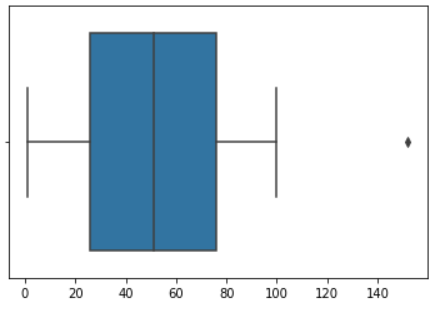
\includegraphics{readme.assets/image-20211210124819306.png}
\caption{image-20211210124819306}
\end{figure}

\hypertarget{uxfcbungen}{%
\chapter{Übungen}\label{uxfcbungen}}

\hypertarget{visualisierungsuxfcbung-1}{%
\section{Visualisierungsübung 1}\label{visualisierungsuxfcbung-1}}

Versuchen sie folgende Kurve zu zeichnen:

\begin{figure}
\centering
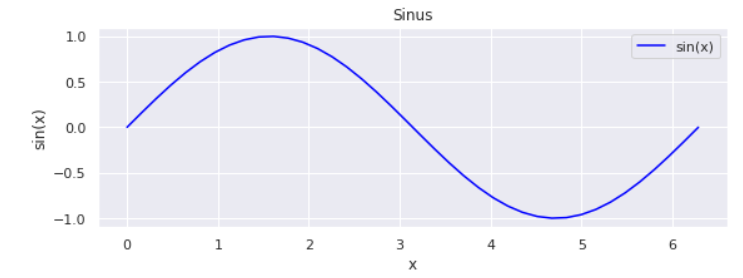
\includegraphics{readme.assets/image-20211210101947217.png}
\caption{image-20211210101947217}
\end{figure}

(Die Lösung finden sie am Ende des Dokumentes)

\hypertarget{visualisierungsuxfcbung-2}{%
\section{Visualisierungsübung 2}\label{visualisierungsuxfcbung-2}}

\begin{enumerate}
\def\labelenumi{\arabic{enumi}.}
\item
  Sie können mit numpy eine Liste mit 50 gleichverteilen Zufallszahlen erstellen. Erzeugen Sie zwei dieser Listen (x und y) und zeigen sie die 50 Paare Paare (x{[}i{]}, y{[}i{]}) in einem Scatterplot an. So ähnlich (!) sollte die Ausgabe aussehen:

  \begin{figure}
  \centering
  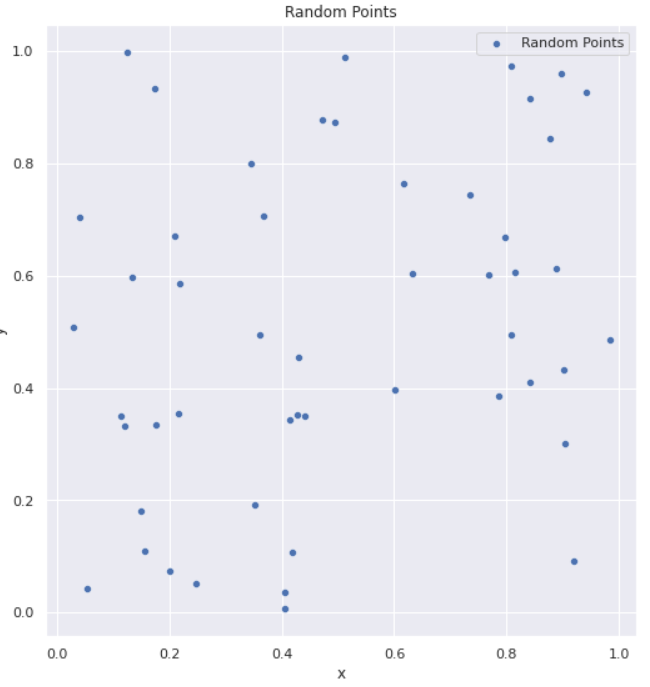
\includegraphics{readme.assets/image-20211210102949673.png}
  \caption{image-20211210102949673}
  \end{figure}
\item
  Welches Ausgabe erwarten Sie, wenn Sie in 1. statt 50 Zahlen jeweils 2000 Zahlen erzeugen? Beschreiben sie das Ergebnis in 2-3 Sätzen.
\item
  Wiederholen sie Aufgabe 1 mit der Normalverteilung (Erwartungswert 0, Standardabweichung 1) statt der Gleichverteilung. Verwenden sie 2000 Punkte. Überlegen sie bitte vorher: welche grafischen Ausgabe erwarten sie?
\item
  Erzeugen Sie ein Histogramm für die Erzeugung von 10000 gleichverteilten (normalverteilten) Zufallszahlen. So ähnlich sollte das Ergebnis aussehen:
\end{enumerate}

\begin{figure}
\centering
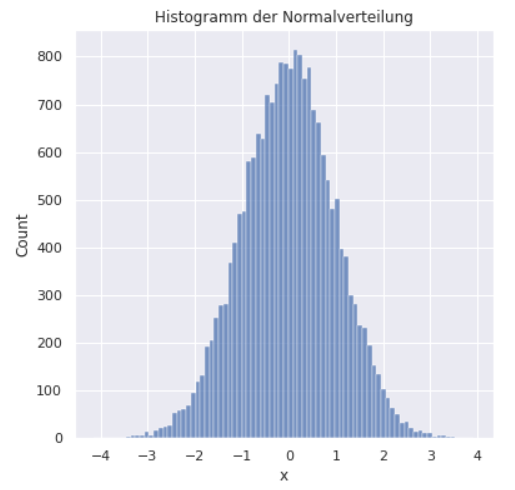
\includegraphics{readme.assets/image-20211210103950590.png}
\caption{image-20211210103950590}
\end{figure}

\hypertarget{plots-fuxfcr-iris}{%
\chapter{Plots für Iris}\label{plots-fuxfcr-iris}}

\hypertarget{laden-der-daten}{%
\section{Laden der Daten}\label{laden-der-daten}}

\begin{verbatim}
import pandas as pd
from sklearn import datasets

import matplotlib.pyplot as plt
import seaborn as sns

iris = datasets.load_iris()
iris_df = pd.DataFrame(iris.data)
iris_df['class']=iris.target_names[iris.target ]
iris_df.columns=['sepal_len', 'sepal_wid', 'petal_len', 'petal_wid', 'class']
\end{verbatim}

\hypertarget{histogramm-fuxfcr-ein-feature}{%
\section{Histogramm für ein Feature}\label{histogramm-fuxfcr-ein-feature}}

\begin{Shaded}
\begin{Highlighting}[]
\NormalTok{sns.}\BuiltInTok{set}\NormalTok{()}
\NormalTok{sns.histplot( iris\_df, }
\NormalTok{             x }\OperatorTok{=}\StringTok{"petal\_wid"}\NormalTok{, }
\NormalTok{             bins}\OperatorTok{=}\DecValTok{10}\NormalTok{,  }\CommentTok{\# try bins="auto" und bins=10}
\NormalTok{             kde }\OperatorTok{=} \VariableTok{False}\NormalTok{)}
\end{Highlighting}
\end{Shaded}

\begin{figure}
\centering
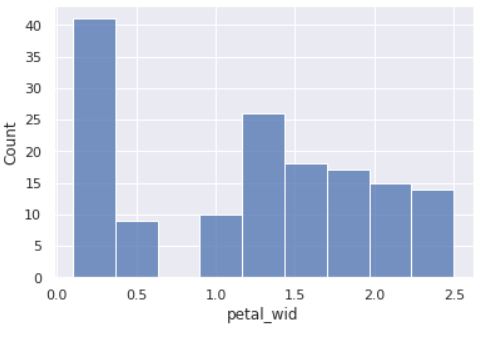
\includegraphics{readme.assets/image-20211209170610859.png}
\caption{image-20211209170610859}
\end{figure}

\hypertarget{relation-plots}{%
\section{Relation-Plots}\label{relation-plots}}

\begin{verbatim}
sns.relplot(data=iris_df, x="petal_len", y="sepal_wid", hue = "class", height=7)
\end{verbatim}

\begin{figure}
\centering
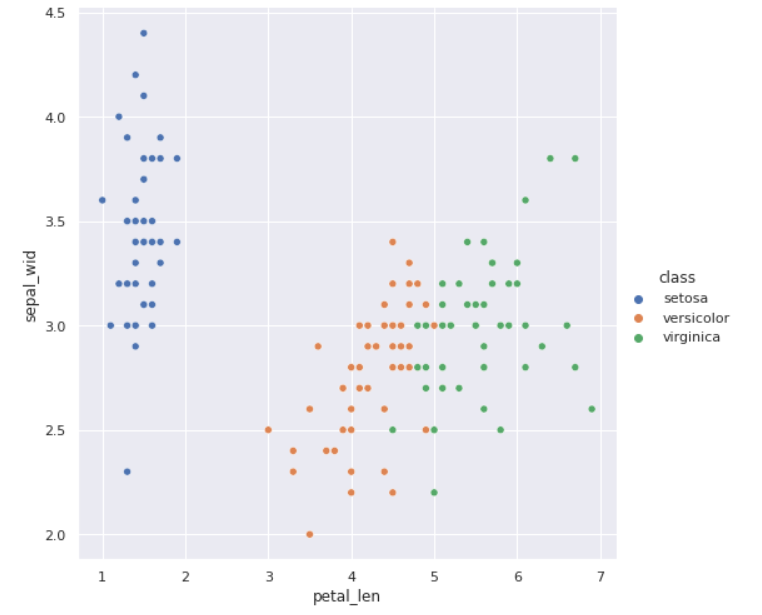
\includegraphics{readme.assets/image-20211209170740088.png}
\caption{image-20211209170740088}
\end{figure}

\hypertarget{pairplots}{%
\section{Pairplots}\label{pairplots}}

\begin{verbatim}
sns.pairplot(iris_df[['sepal_len', 'sepal_wid', 'petal_len', 'petal_wid', 'class']],
             hue="class", diag_kind="kde")
\end{verbatim}

Ausgabe:

\begin{figure}
\centering
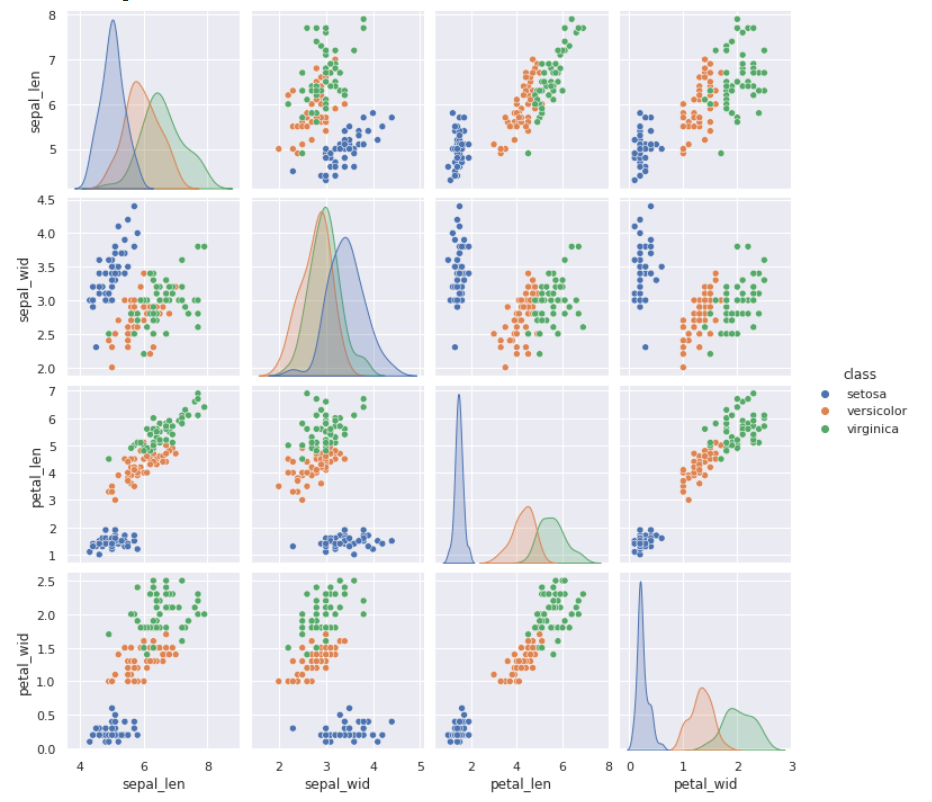
\includegraphics{readme.assets/image-20211209171426965.png}
\caption{image-20211209171426965}
\end{figure}

\hypertarget{beispiele-bilder}{%
\chapter{Beispiele: Bilder}\label{beispiele-bilder}}

Bilder lassen sich als Numpy-Arrays darstellen und bearbeiten. Unterstützte shapes sind:

\begin{itemize}
\tightlist
\item
  (M, N): ein Bild mit skalaren Werten (0-1 float oder 0-255 int). Visualisierung erfolgt über eine \emph{colormap}.
\item
  (M, N, 3): ein Farbbild mit RGB Werten (0-1 float oder 0-255 int).
\end{itemize}

Die ersten beiden Werte (M, N) definieren die Anzahl der Zeilen und Spalten des Bildes.

(Taken from \url{https://matplotlib.org/3.1.1/api/_as_gen/matplotlib.pyplot.imshow.html})

\hypertarget{grauwert-bilder-als-nxm-matrix}{%
\section{Grauwert-Bilder als nxm Matrix}\label{grauwert-bilder-als-nxm-matrix}}

Folgende Befehle erzeugen ein künstliches und (gleichverteilt) zufälliges Grauwertbild:

\begin{Shaded}
\begin{Highlighting}[]
\ImportTok{import}\NormalTok{ matplotlib.pyplot }\ImportTok{as}\NormalTok{ plt}
\ImportTok{import}\NormalTok{ numpy }\ImportTok{as}\NormalTok{ np}

\NormalTok{img }\OperatorTok{=}\NormalTok{ np.random.rand(}\DecValTok{10}\NormalTok{,}\DecValTok{10}\NormalTok{)}
\NormalTok{plt.imshow(img, cmap}\OperatorTok{=}\NormalTok{ plt.cm.get\_cmap(}\StringTok{\textquotesingle{}Oranges\textquotesingle{}}\NormalTok{), vmin}\OperatorTok{=}\DecValTok{0}\NormalTok{, vmax}\OperatorTok{=}\DecValTok{1}\NormalTok{  )}
\end{Highlighting}
\end{Shaded}

Colormaps finden sie unter \url{https://matplotlib.org/3.1.0/tutorials/colors/colormaps.html}. Sie können auch probieren: `Greys', `Purples', `Blues', `Greens', `Oranges', `Reds', `YlOrBr', `YlOrRd', `OrRd', `PuRd', `RdPu', `BuPu', `GnBu', `PuBu', `YlGnBu', `PuBuGn', `BuGn', `YlGn'

\hypertarget{farbbilder-aus-datei-laden}{%
\section{Farbbilder aus Datei laden}\label{farbbilder-aus-datei-laden}}

\begin{Shaded}
\begin{Highlighting}[]
\ImportTok{import}\NormalTok{ numpy }\ImportTok{as}\NormalTok{ np}
\ImportTok{import}\NormalTok{ matplotlib.pyplot }\ImportTok{as}\NormalTok{ plt}

\NormalTok{url }\OperatorTok{=} \StringTok{\textquotesingle{}http://www.dietergreipl.de/wp{-}content/uploads/2019/10/owl{-}50267\_1920.png\textquotesingle{}}
\NormalTok{eule }\OperatorTok{=}\NormalTok{ plt.imread( url )}
\BuiltInTok{print}\NormalTok{(eule.shape)}
\BuiltInTok{print}\NormalTok{(np.amax( eule ))}
\BuiltInTok{print}\NormalTok{(np.amin( eule ))}
\NormalTok{plt.figure( figsize}\OperatorTok{=}\NormalTok{(}\DecValTok{20}\NormalTok{,}\DecValTok{15}\NormalTok{))}
\NormalTok{plt.imshow( eule )}
\end{Highlighting}
\end{Shaded}

\begin{figure}
\centering
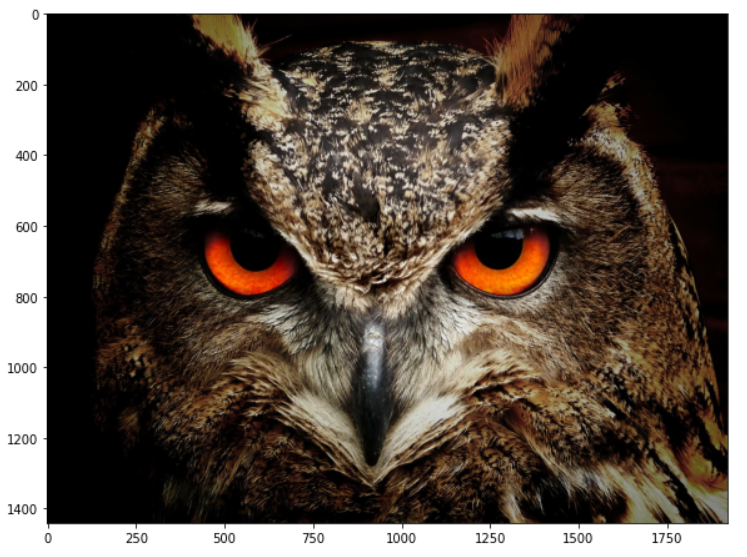
\includegraphics{readme.assets/image-20211210112329871.png}
\caption{image-20211210112329871}
\end{figure}

\hypertarget{einfache-farbbilder-erzeugen}{%
\section{Einfache Farbbilder erzeugen}\label{einfache-farbbilder-erzeugen}}

\begin{Shaded}
\begin{Highlighting}[]
\ImportTok{import}\NormalTok{ numpy }\ImportTok{as}\NormalTok{ np}
\ImportTok{import}\NormalTok{ matplotlib.pyplot }\ImportTok{as}\NormalTok{ plt}
\NormalTok{img }\OperatorTok{=}\NormalTok{ np.zeros( (}\DecValTok{200}\NormalTok{,}\DecValTok{200}\NormalTok{,}\DecValTok{3}\NormalTok{))}
\NormalTok{img[:,:,}\DecValTok{1}\NormalTok{] }\OperatorTok{=}\NormalTok{ np.ones((}\DecValTok{200}\NormalTok{))}
\NormalTok{plt.figure()}
\NormalTok{plt.imshow( img  )}
\end{Highlighting}
\end{Shaded}

\hypertarget{komplett-zufuxe4lliges-farbbild}{%
\section{Komplett zufälliges Farbbild}\label{komplett-zufuxe4lliges-farbbild}}

\begin{Shaded}
\begin{Highlighting}[]
\ImportTok{import}\NormalTok{ numpy }\ImportTok{as}\NormalTok{ np}
\ImportTok{import}\NormalTok{ matplotlib.pyplot }\ImportTok{as}\NormalTok{ plt}
\NormalTok{img }\OperatorTok{=}\NormalTok{ np.random.random( }\DecValTok{200}\OperatorTok{*}\DecValTok{200}\OperatorTok{*}\DecValTok{3}\NormalTok{).reshape(}\DecValTok{200}\NormalTok{,}\DecValTok{200}\NormalTok{,}\DecValTok{3}\NormalTok{)}
\NormalTok{plt.figure(figsize}\OperatorTok{=}\NormalTok{ (}\DecValTok{9}\NormalTok{,}\DecValTok{9}\NormalTok{))}
\NormalTok{plt.imshow( img  )}
\end{Highlighting}
\end{Shaded}

\begin{figure}
\centering
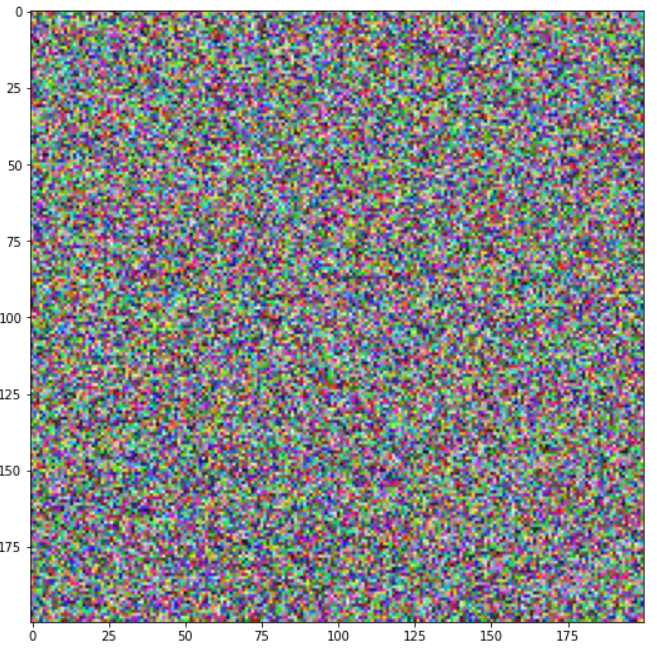
\includegraphics{readme.assets/image-20211210112144985.png}
\caption{image-20211210112144985}
\end{figure}

\hypertarget{uxfcbungen-1}{%
\subsection{Übungen}\label{uxfcbungen-1}}

\hypertarget{wie-kommt-dieses-bild-zustande}{%
\subsubsection{Wie kommt dieses Bild zustande?}\label{wie-kommt-dieses-bild-zustande}}

Erläutern Sie, wie das Bild erstellt wird, speziell die for-Schleife:

\begin{Shaded}
\begin{Highlighting}[]
\ImportTok{import}\NormalTok{ numpy }\ImportTok{as}\NormalTok{ np}
\ImportTok{import}\NormalTok{ matplotlib.pyplot }\ImportTok{as}\NormalTok{ plt}

\NormalTok{img}\OperatorTok{=}\NormalTok{ np.ones((}\DecValTok{200}\NormalTok{, }\DecValTok{200}\NormalTok{))}

\ControlFlowTok{for}\NormalTok{ col }\KeywordTok{in} \BuiltInTok{range}\NormalTok{(}\DecValTok{0}\NormalTok{, }\DecValTok{200}\NormalTok{):}
\NormalTok{  img[:,col] }\OperatorTok{=}\NormalTok{ col}

\NormalTok{plt.figure(figsize}\OperatorTok{=}\NormalTok{ (}\DecValTok{9}\NormalTok{,}\DecValTok{9}\NormalTok{))}
\NormalTok{plt.imshow( img, cmap}\OperatorTok{=}\NormalTok{ plt.get\_cmap(}\StringTok{\textquotesingle{}gray\textquotesingle{}}\NormalTok{), vmin}\OperatorTok{=}\DecValTok{0}\NormalTok{, vmax}\OperatorTok{=}\DecValTok{200}\NormalTok{)}
\end{Highlighting}
\end{Shaded}

Ausgabe:

\begin{figure}
\centering
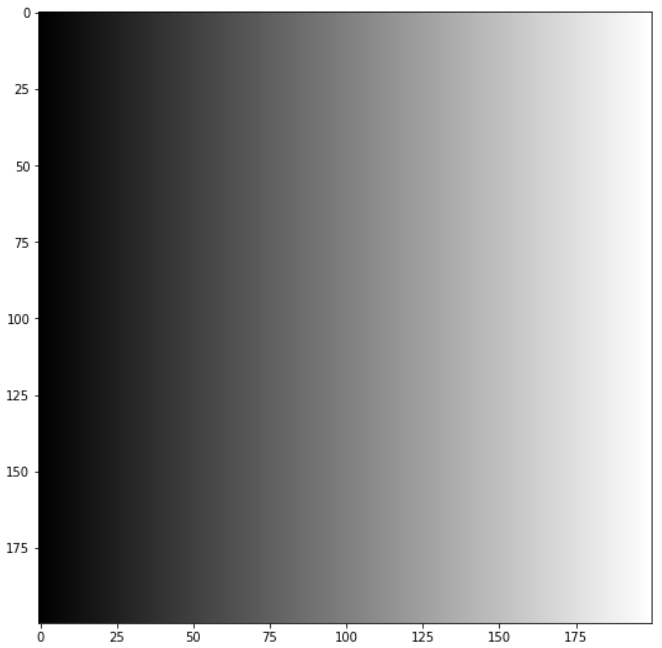
\includegraphics{readme.assets/image-20211210112001756.png}
\caption{image-20211210112001756}
\end{figure}

\hypertarget{erkluxe4ren-sie-die-ausgabe-dieses-programms}{%
\subsubsection{Erklären sie die Ausgabe dieses Programms:}\label{erkluxe4ren-sie-die-ausgabe-dieses-programms}}

\begin{verbatim}
import numpy as np
import matplotlib.pyplot as plt
img = np.random.normal(0.5, 0.1, 200*200*3).reshape(200,200,3)
plt.figure(figsize= (9,9))
plt.imshow( img  )
\end{verbatim}

Ausgabe:

\begin{figure}
\centering
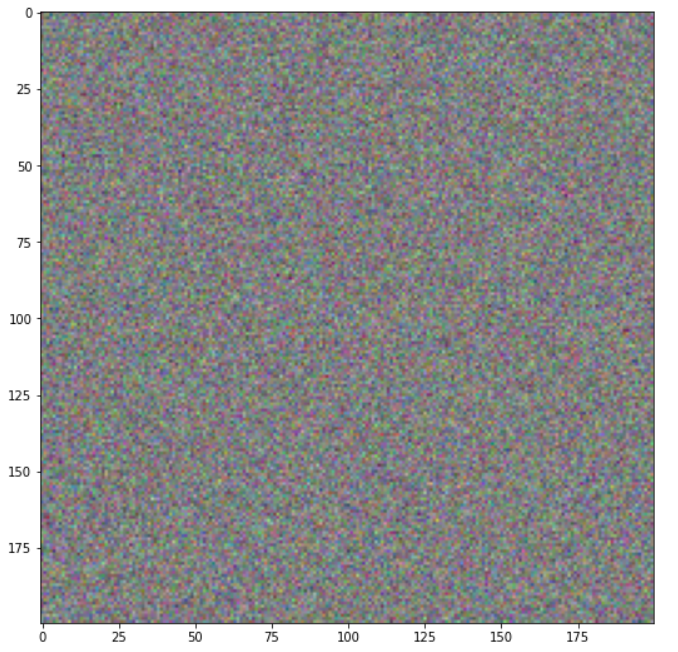
\includegraphics{readme.assets/image-20211210113514004.png}
\caption{image-20211210113514004}
\end{figure}

\hypertarget{sandbox}{%
\chapter{Sandbox}\label{sandbox}}

\hypertarget{alle-farben}{%
\section{Alle Farben}\label{alle-farben}}

Folgendes Programm gibt alle Farben mit Farbnamen aus:

\begin{verbatim}
from matplotlib.patches import Rectangle
import matplotlib.pyplot as plt
import matplotlib.colors as mcolors


def plot_colortable(colors, title, sort_colors=True, emptycols=0):

    cell_width = 212
    cell_height = 22
    swatch_width = 48
    margin = 12
    topmargin = 40

    # Sort colors by hue, saturation, value and name.
    if sort_colors is True:
        by_hsv = sorted((tuple(mcolors.rgb_to_hsv(mcolors.to_rgb(color))),
                         name)
                        for name, color in colors.items())
        names = [name for hsv, name in by_hsv]
    else:
        names = list(colors)

    n = len(names)
    ncols = 4 - emptycols
    nrows = n // ncols + int(n % ncols > 0)

    width = cell_width * 4 + 2 * margin
    height = cell_height * nrows + margin + topmargin
    dpi = 72

    fig, ax = plt.subplots(figsize=(width / dpi, height / dpi), dpi=dpi)
    fig.subplots_adjust(margin/width, margin/height,
                        (width-margin)/width, (height-topmargin)/height)
    ax.set_xlim(0, cell_width * 4)
    ax.set_ylim(cell_height * (nrows-0.5), -cell_height/2.)
    ax.yaxis.set_visible(False)
    ax.xaxis.set_visible(False)
    ax.set_axis_off()
    ax.set_title(title, fontsize=24, loc="left", pad=10)

    for i, name in enumerate(names):
        row = i % nrows
        col = i // nrows
        y = row * cell_height

        swatch_start_x = cell_width * col
        text_pos_x = cell_width * col + swatch_width + 7

        ax.text(text_pos_x, y, name, fontsize=14,
                horizontalalignment='left',
                verticalalignment='center')

        ax.add_patch(
            Rectangle(xy=(swatch_start_x, y-9), width=swatch_width,
                      height=18, facecolor=colors[name], edgecolor='0.7')
        )

    return fig

plot_colortable(mcolors.BASE_COLORS, "Base Colors",
                sort_colors=False, emptycols=1)
plot_colortable(mcolors.TABLEAU_COLORS, "Tableau Palette",
                sort_colors=False, emptycols=2)

plot_colortable(mcolors.CSS4_COLORS, "CSS Colors")

# Optionally plot the XKCD colors (Caution: will produce large figure)
# xkcd_fig = plot_colortable(mcolors.XKCD_COLORS, "XKCD Colors")
# xkcd_fig.savefig("XKCD_Colors.png")

plt.show()
\end{verbatim}

\hypertarget{luxf6sungen}{%
\section{Lösungen}\label{luxf6sungen}}

\hypertarget{visualisierung-1}{%
\subsection{Visualisierung 1}\label{visualisierung-1}}

\begin{Shaded}
\begin{Highlighting}[]
\ImportTok{import}\NormalTok{ matplotlib.pyplot }\ImportTok{as}\NormalTok{ plt}
\ImportTok{import}\NormalTok{ seaborn }\ImportTok{as}\NormalTok{ sns}
\ImportTok{import}\NormalTok{ numpy }\ImportTok{as}\NormalTok{ np}

\NormalTok{x }\OperatorTok{=}\NormalTok{ np.linspace(}\DecValTok{0}\NormalTok{, }\DecValTok{2}\OperatorTok{*}\NormalTok{np.pi, }\DecValTok{40}\NormalTok{)}

\NormalTok{fig,ax }\OperatorTok{=}\NormalTok{ plt.subplots(figsize}\OperatorTok{=}\NormalTok{(}\DecValTok{9}\NormalTok{, }\DecValTok{9}\NormalTok{))}

\NormalTok{ax.set\_title(}\StringTok{"Sinus"}\NormalTok{) }
\NormalTok{ax.set\_xlabel(}\StringTok{"x"}\NormalTok{)}
\NormalTok{ax.set\_ylabel(}\StringTok{"sin(x)"}\NormalTok{)}
\NormalTok{ax.set\_aspect(}\StringTok{"equal"}\NormalTok{)}

\NormalTok{sns.}\BuiltInTok{set}\NormalTok{()}
\NormalTok{sns.lineplot(x}\OperatorTok{=}\NormalTok{x, y}\OperatorTok{=}\NormalTok{ np.sin(x), color}\OperatorTok{=}\StringTok{"blue"}\NormalTok{, label}\OperatorTok{=}\StringTok{"sin(x)"}\NormalTok{)}
\end{Highlighting}
\end{Shaded}

\hypertarget{visualisierung-2}{%
\subsection{Visualisierung 2}\label{visualisierung-2}}

\hypertarget{section}{%
\subsubsection{2.1}\label{section}}

\begin{Shaded}
\begin{Highlighting}[]
\ImportTok{import}\NormalTok{ matplotlib.pyplot }\ImportTok{as}\NormalTok{ plt}
\ImportTok{import}\NormalTok{ seaborn }\ImportTok{as}\NormalTok{ sns}
\ImportTok{import}\NormalTok{ numpy }\ImportTok{as}\NormalTok{ np}

\NormalTok{x }\OperatorTok{=}\NormalTok{ np.random.random(}\DecValTok{50}\NormalTok{)}
\NormalTok{y }\OperatorTok{=}\NormalTok{ np.random.random(}\DecValTok{50}\NormalTok{)}

\NormalTok{fig,ax }\OperatorTok{=}\NormalTok{ plt.subplots(figsize}\OperatorTok{=}\NormalTok{(}\DecValTok{9}\NormalTok{, }\DecValTok{9}\NormalTok{))}

\NormalTok{sns.}\BuiltInTok{set}\NormalTok{()}
\NormalTok{ax.set\_title(}\StringTok{"Random Points"}\NormalTok{) }
\NormalTok{ax.set\_xlabel(}\StringTok{"x"}\NormalTok{)}
\NormalTok{ax.set\_ylabel(}\StringTok{"y"}\NormalTok{)}
\NormalTok{ax.set\_aspect(}\StringTok{"equal"}\NormalTok{)}

\NormalTok{sns.scatterplot(x}\OperatorTok{=}\NormalTok{x, y}\OperatorTok{=}\NormalTok{y, label}\OperatorTok{=}\StringTok{"Random Points"}\NormalTok{)}
\end{Highlighting}
\end{Shaded}

\hypertarget{section-1}{%
\subsubsection{2.3}\label{section-1}}

\begin{verbatim}
import matplotlib.pyplot as plt
import seaborn as sns
import numpy as np

x = np.random.normal(0,1,2000)
y = np.random.normal(0,1,2000)

fig,ax = plt.subplots(figsize=(9, 9))

sns.set()
ax.set_title("Random Points") 
ax.set_xlabel("x")
ax.set_ylabel("y")
ax.set_aspect("equal")

sns.scatterplot(x=x, y=y, label="Random Points")
\end{verbatim}

\hypertarget{section-2}{%
\subsubsection{2.4}\label{section-2}}

\begin{Shaded}
\begin{Highlighting}[]
\ImportTok{import}\NormalTok{ matplotlib.pyplot }\ImportTok{as}\NormalTok{ plt}
\ImportTok{import}\NormalTok{ seaborn }\ImportTok{as}\NormalTok{ sns}
\ImportTok{import}\NormalTok{ numpy }\ImportTok{as}\NormalTok{ np}

\NormalTok{x }\OperatorTok{=}\NormalTok{ np.random.normal(}\DecValTok{0}\NormalTok{,}\DecValTok{1}\NormalTok{,}\DecValTok{20000}\NormalTok{)}


\NormalTok{fig,ax }\OperatorTok{=}\NormalTok{ plt.subplots(figsize}\OperatorTok{=}\NormalTok{(}\DecValTok{6}\NormalTok{, }\DecValTok{6}\NormalTok{))}

\NormalTok{sns.}\BuiltInTok{set}\NormalTok{()}
\NormalTok{ax.set\_title(}\StringTok{"Histogramm der Normalverteilung"}\NormalTok{) }
\NormalTok{ax.set\_xlabel(}\StringTok{"x"}\NormalTok{)}
\NormalTok{ax.set\_ylabel(}\StringTok{"Count"}\NormalTok{)}

\NormalTok{sns.histplot(x}\OperatorTok{=}\NormalTok{x)}
\end{Highlighting}
\end{Shaded}


  \bibliography{book.bib,packages.bib}

\end{document}
